\section{Iterační metody řešení soustav lineárních rovnic}

V této kapitole se budeme zabývat numerickým řešením soustavy
$$ \A\xx=\bb. $$
Předpokládáme, že čtenáři je známa Gaussova eliminační metoda, která je pří\-kla\-dem tzv. přímých metod.
Její výhodou je univerzálnost --- metoda vyřeší v přesné aritmetice soustavu s libovolnou regulární maticí.
Nevýhodou je její neefektivita pro velké matice a také to, že v průběhu výpočtu nemá uživatel žádnou informaci o výsledku.
Pro úlohy s velkou řídkou maticí $\A$, se kterými se setkáváme v mnoha praktických problémech, nebo pro úlohy, kde matice není dána explicitně nebo je drahé ji sestavit, může být výhodou použít iterační metody.
Tyto metody v zásadě používají jen násobení matic a v průběhu výpočtu postupně vylepšují aproximaci přesného řešení.
Konvergence iteračního procesu může být asymptotická nebo v konečném počtu iterací.

Pro detaily ohledně odvození a dalších vlastností iteračních metod odkazujeme na knihu \cite{analyza_metod_maticove_vyp}.



\subsection{Klasické iterační metody}

Klasické iterační metody jsou založeny na štěpení matice soustavy $\A = \mat M + \mat N$ takovém, že matice $\mat M$ je regulární a snadno invertovatelná a $\mat M$ a $\mat N$ jsou zvoleny nějakým vhodným způsobem.
Dosazením tohoto štěpení do vztahu $\mat A\xx = \bb$ dostáváme $(\mat M + \mat N)\xx = \bb$ a odtud
$$ \xx = \mat M^{-1}(\bb - \mat N\xx) = \mat M^{-1}(\bb + \mat M\xx - \mat A\xx) = \xx + \mat M^{-1}(\bb - \mat A\xx). $$
Je-li dána počáteční aproximace řešení $\xx_0$, můžeme definovat iterační proces následovně:
$$ \xx_k = \xx_{k-1} + \mat M^{-1} (\bb - \mat A\xx_{k-1} )
= (\I - \mat M^{-1}\mat A)\xx_{k-1} + \mat M^{-1}\bb. $$
Lze ukázat, že pro chybu aproximace platí odhad
$$ \frac{\norm{\xx-\xx_k}}{\norm{\xx-\xx_0}} \le \norm{(\I-\mat M^{-1}\A)^k} \le \norm{\I-\mat M^{-1}\A}^k, $$
přičemž pro velká $k$ je $\norm{(\I-\mat M^{-1}\A)^k}\approx\rho(\I-\mat M^{-1}\A)^k$ (symbolem $\rho(\A)$ značíme tzv. spektrální poloměr, který je definován jako $\max\{|\lambda|;~\lambda\in\sigma(\A)\}$).
Vidíme tedy, že metody konvergují k přesnému řešení, pokud $\rho(\I-\mat M^{-1}\A)<1$.
I v případě, že tato podmínka je splněna, však může být $\norm{\I-\mat M^{-1}\A}^k>1$ a dochází pak k tzv. přechodovému jevu, kdy chyba aproximace nejprve roste a teprve pak začne klesat (viz obr. \ref{fig:prechod}).
\begin{figure}
\centering
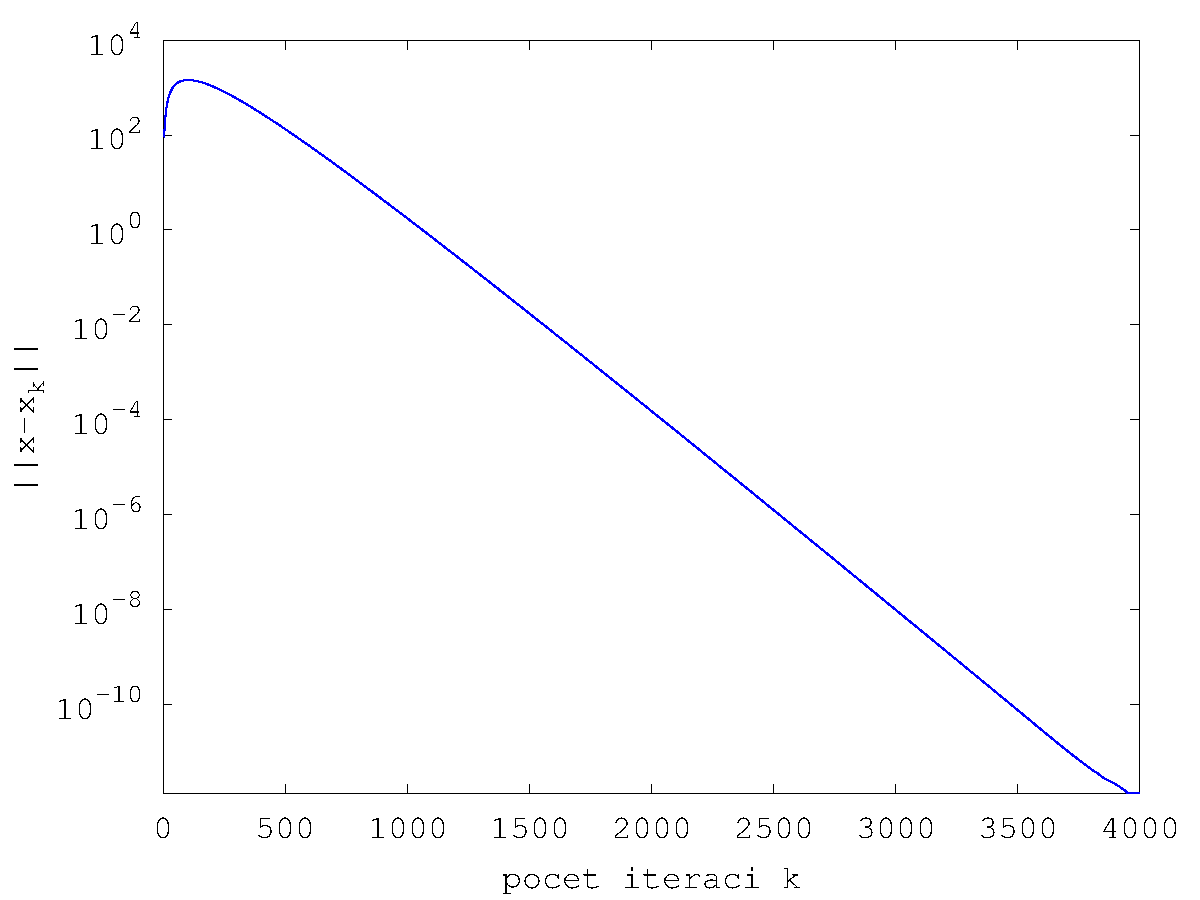
\includegraphics[width=6cm]{img/prechod}
\caption{Přechodový jev u klasické iterační metody.}
\label{fig:prechod}
\end{figure}


\paragraph{Příklady klasických iteračních metod.}
Následující metody jsou založeny na štěpení $\A=\mat D-\mat L-\mat U$, kde $\mat D$ je hlavní diagonála, $-\mat L$ je striktně dolní trojúhelník matice $\A$ a $-\mat U$ je striktně horní trojúhelník.
Z rovnice
$$ (\mat D-\mat L-\mat U)\xx=\bb $$
pak lze odvodit jednotlivé metody.

{\bf Jacobiova metoda} je definována iterací
$$ \mat D\xx_k=\mat L\xx_{k-1} + \mat U\xx_{k-1} + \bb. $$
Rozepíšeme-li tento vzorec po složkách ($x_i^k$ značí $i$-tou složku vektoru $\xx_k$), dostaneme pro $i=1,\ldots,n$:
$$ x_i^k = \frac1{a_{ii}}\left(b_i-\sum_{j=1,j\neq i}^n a_{ij}x_j^{k-1}\right). $$
Nevýhodou této metody může být, že v průběhu výpočtu je třeba uchovávat dvě posobě jdoucí aproximace řešení $\xx_k$, $\xx_{k-1}$.
Metoda {\bf Gauss-Seidelova} se od předchozí liší v tom, že ihned využívá již spočtené složky vektoru $\xx_k$, tj. po složkách počítá
$$ x_i^k = \frac1{a_{ii}}\left(b_i-\sum_{j=1}^{i-1} a_{ij}x_j^k-\sum_{j=i+1}^n a_{ij}x_j^{k-1}\right). $$
Spočtené složky aproximace řešení je tedy možné ihned přepisovat.
Maticově lze tuto iteraci zapsat jako
$$ \mat D\xx_k=\mat L\xx_k+\mat U\xx_{k-1}+\bb. $$
Z Gauss-Seidelovy metody je odvozena {\bf Superrelaxační metoda} (SOR, successive over-relaxation).
Pracuje s relaxačním parametrem $\omega\in[0,2]$ a je definována vztahem
$$ \mat D\xx_k = \omega(\mat L\xx_k+\mat U\xx_{k-1}+\bb) + (1-\omega)\mat D\xx_{k-1}, $$
tj. kombinuje Gauss-Seidelovu metodu s předchozí iterací.
\begin{ex}
Uvažujme matici
\[ \A = \begin{pmatrix}0.01 & -0.4\\0&0.01\end{pmatrix}. \]
Konvergence Jacobiovy metody pro tuto matici závisí na vlastnostech matice
\[ \I - \mat D^{-1}\A = \begin{pmatrix}0&-40\\0&0\end{pmatrix}. \]
Jelikož tato matice má pouze nulové vlastní číslo, její spektrální poloměr je $0$, a tedy podmínka $\rho(\I-\mat D^{-1}\A)<1$ je splněna, neboli metoda konverguje.
Na druhé straně $\norm{\I-\mat D^{-1}\A}=40>1$, při výpočtu proto lze pozorovat přechodový jev.
\end{ex}






\subsection{Metody Krylovových podprostorů}

Důležitá třída iteračních metod je založena na myšlence projektovat soustavu $\A\xx=\bb$ na posloupnost tzv. Krylovových prostorů a tím získávat postupně aproximace řešení.
\begin{df}
Nechť $\A\in\R^{n\times n}$, $\vv\in\R^n$ a $k\le n$.
$k$-tým Krylovovým prostorem nazýváme podprostor
$$ \mathcal K_k(\A,\vv):=\lo{\vv,\A\vv,\A^2\vv,\ldots,\A^{k-1}\vv}. $$
\end{df}
Metody, které zmíníme v následující části, mají společnou vlastnost tzv. projekčních metod, tj. hledají aproximace ve tvaru
$$ \xx_k\in \xx_0 + \mathcal S_k, \quad \rr_k\perp\mathcal C_k, $$
kde $\rr_k:=\bb-\A\xx_k$ je tzv. reziduum a $\mathcal S_k$ a $\mathcal C_k$ jsou vhodné podprostory.
Prostor $\mathcal S_k$ je obvykle roven Krylovovu podprostoru $\mathcal K_k(\A,\rr_0)$, ale jsou možné i jiné volby, např. $\A\mathcal K_k(\A,\rr_0)$.
Volbou prostoru $\mathcal C_k$ lze docílit optimality aproximace řešení v tom smyslu, že chyba aproximace $\xx-\xx_k$ je v nějaké normě minimální.
Pokud dimenze podprostorů $\mathcal S_k$, $\mathcal C_k$ roste, pak pro $k=n$ dostáváme $\mathcal C_n=\R^n$ a z podmínky $\rr_k\perp\mathcal\R^n$ plyne $\rr_n=\0$, tedy $\xx_n=\xx$ je přesné řešení.
Jinak řečeno, rostou-li dimenze prostorů $\mathcal S_k$, $\mathcal C_k$, pak projekční metody najdou řešení systému $\A\xx=\bb$ nejvýše v $n$ krocích.


\subsubsection{Metoda sdružených gradientů (CG)}
\label{sec:cg}

Tato metoda (stručně ji budeme označovat symbolem CG --- z anglického \emph{Conjugate gradients}) je určena pro symetrické pozitivně definitní matice.
\begin{df}
Matice $\A\in\R^{n\times n}$ je pozitivně definitní, pokud pro každý nenulový vektor $\xx\in\R^n$ platí:
$$ \A\xx\cdot\xx>0. $$
Výraz
$$ \norm{\xx}_\A:=\sqrt{\xx\cdot\A\xx} $$
se nazývá energetická norma nebo také $\A$-norma.
Řekneme, že vektory $\uu,\vv\in\R^n$ jsou navzájem $\A$-ortogonální, jestliže
$$ \uu\cdot\A\vv=0. $$
\end{df}
Aproximace řešení je v metodě CG konstruována podle vzorce
$$ \xx_k:=\xx_{k-1}+\gamma_{k-1}\pp_{k-1}, $$
kde $\pp_{k-1}$ je směrový vektor a $\gamma_{k-1}$ je délka kroku.
Tyto parametry se určí následujícím způsobem:
\begin{itemize}
\item $\pp_k$ volíme ve tvaru $\pp_k:=\rr_k+\delta_k\pp_{k-1}$ tak, aby byl $\A$-ortogonální na $\pp_{k-1}$, tj. $\pp_k\cdot\A\pp_{k-1}=0$. Toho docílíme pro
$$ \delta_k:=\frac{\rr_k\cdot\rr_k}{\rr_{k-1}\cdot\rr_{k-1}}. $$
\item $\gamma_{k-1}$ volíme takové, aby byla minimální energetická norma $\norm{\xx-\xx_k}_\A$. To nastane právě tehdy, když
$$ \gamma_{k-1}:=\frac{\rr_{k-1}\cdot\rr_{k-1}}{\pp_{k-1}\cdot\A\pp_{k-1}}. $$
\end{itemize}
Na základě předchozích vztahů lze ukázat že CG patří mezi Krylovovské metody, neboť platí:
$$ \xx_k\in\xx_0+\mathcal K_k(\A,\rr_0),\quad \rr_k\perp\mathcal K_k(\A,\rr_0). $$
Na metodu sdružených gradientů lze také nahlížet jako na metodu, která hledá mi\-ni\-mum kvadratického funkcionálu $\frac12\xx\cdot\A\xx-\xx\cdot\bb$.
Následující algoritmus reprezentuje standardní implementaci metody CG.

\algoritmus{Metoda sdružených gradientů}{
{\bf input} $\A$, $\bb$, $\xx_0$\\
$\rr_0:=\bb-\A\xx_0$\\
$\pp_0:=\rr_0$\\
{\bf for }$k=1,2,\ldots$\\
$\quad \gamma_{k-1}:=\frac{\rr_{k-1}\cdot\rr_{k-1}}{\pp_{k-1}\cdot\A\pp_{k-1}}$\\
$\quad \xx_k:=\xx_{k-1}+\gamma_{k-1}\pp_{k-1}$\\
$\quad \rr_k:=\rr_{k-1}-\gamma_{k-1}\A\pp_{k-1}$\\
$\quad \delta_k:=\frac{\rr_k\cdot\rr_k}{\rr_{k-1}\cdot\rr_{k-1}}$\\
$\quad \pp_k:=\rr_k+\delta_k\pp_{k-1}$\\
{\bf end}
}

Vidíme, že v každé iteraci je třeba provést 1 násobení matice $\A$ s vektorem a v průběhu výpočtu je třeba uchovávat pouze 4 vektory.
Metoda CG je tedy velmi efektivní zejména pro velké řídké matice.
Je-li matice symetrická pozitivně definitní, pak v přesné aritmetice algoritmus nalezne řešení nejvýše po $n$ iteracích.
V praxi ovšem kvůli zaokrouhlovacím chybám dochází ke ztrátě $\A$-ortogonality vektorů $\{\pp_k\}$ (resp. ortogonality vektorů $\{\rr_k\}$), což způsobuje zpoždění konvergence, tedy že i po $n$ krocích je $\xx_n\neq\xx$.
Tento nedostatek se někdy odstraňuje tak, že se vektor $\rr_k$ ortogonalizuje proti všem předchozím $\{\rr_i\}_{i=0}^{k-1}$ a proces ortogonalizace se zopakuje vícekrát (obvykle stačí dvakrát).

Nyní si uvedeme, co je známo o rychlosti konvergence metody CG.
K tomu potřebujeme znát pojem \emph{číslo podmíněnosti}.
\begin{df}
Nechť $\A$ je symetrická pozitivně definitní matice.
Číslo podmíněnosti matice $\A$ je definováno předpisem
$$ \varkappa(\A):=\frac{\lambda_{max}(\A)}{\lambda_{min}(\A)}, $$
kde $\lambda_{max}(\A)$, $\lambda_{min}(\A)$ značí největší, resp. nejmenší vlastní číslo matice $\A$.
\end{df}
Označíme-li $\ee_k:=\xx_k-\xx$ chybu $k$-té aproximace řešení, pak platí následující odhad chyby:
$$ \frac{\norm{\ee_k}_\A}{\norm{\ee_0}_\A} \le 2\left(\frac{\sqrt{\varkappa(\A)}-1}{\sqrt{\varkappa(\A)}+1}\right)^k. $$
Všimněme si, že číslo v závorce v předchozí nerovnosti je vždy menší než $1$.
Pokud je $\varkappa(\A)$ blízké $1$, pak odhad chyby říká, že chyba klesá velmi rychle.
Pro špatně podmíněné matice (tj. je-li $\varkappa(\A)$ velké) je číslo v závorce blízké jedné a odhad často nadhodnocuje skutečnou velikost $\A$-normy chyby.
Špatná podmíněnost matice přesto může mít za následek pomalou konvergenci metody.
Tuto skutečnost lze řešit pomocí tzv. předpodmínění, které spočívá v tom, že původní soustava $\A\xx=\bb$ se nahradí ekvivalentní soustavou $\hat\A\hat\xx=\hat\bb$ s maticí $\hat\A$, která má menší číslo podmíněnosti než $\A$.



% sdružené gradienty - zastavovací kritéria, počáteční aproximace
\subsubsection{Zobecněná metoda minimálních reziduí (GMRES)}

Metodu GMRES (generalized minimal residual method) lze charakterizovat ve smyslu projekčních metod pomocí vztahů
$$ \xx_k\in\xx_0+\mathcal K_k(\A,\rr_0),\quad \rr_k\perp\A\mathcal K_k(\A,\rr_0). $$
Jak napovídá název, její vlastností je, že v každé iteraci minimalizuje normu rezidua $\norm{\rr_k}$.
To vede na úlohu nejmenších čtverců, jejíž efektivní implementace je poměrně technicky obtížná.
Proto zde její algoritmus neuvádíme.
Nepříjemnou vlastností metody GMRES je, že produkuje posloupnost ortogonálních vektorů $\{\vv_k\}$, které je třeba uchovávat, (říkáme, že metoda generuje dlouhé rekurence) a to klade vysoké nároky na paměť.
Za tuto cenu ovšem metoda dokáže řešit soustavu s libovolnou regulární maticí.

% \algoritmus{Zobecněná metoda minimálních reziduí (GMRES)}{
% {\bf input} $\A$, $\bb$, $\xx_0$\\
% $\rr_0:=\bb-\A\xx_0$\\
% $\vv_1:=\rr_0/\norm{\rr_0}$\\
% {\bf for }$k=1,2,\ldots$\\
% \quad$\ww:=\A\vv_k$\\
% \quad{\bf for }$i=1,\ldots,k$\\
% \qquad $h_{i,k}:=\vv_i\cdot\ww$\\
% \qquad $\ww:=\ww- h_{i,k}\vv_i$\\
% \quad{\bf end}\\
% \quad$h_{k+1,k}:=\norm{\ww}$\\
% 
% {\bf end}
% }

Stejně jako u metody CG, vlivem zaokrouhlovacích chyb dochází ke zpomalení konvergence kvůli ztrátě ortogonality systému $\{\vv_k\}$.
I u GMRES tedy obvykle provádíme vícenásobnou ortogonalizaci.
Problém s paměťovou náročností se obvykle řeší pomocí tzv. restartu --- program uchovává místo celé posloupnosti jen posledních $m$ vektorů $\{\vv_i\}_{i=k-m+1}^k$.



% GMRES - charakteristika, schéma algoritmu, vlastnosti - obecná regulární matice, dlouhé rekurence, ztráta ortogonality, restart

\subsubsection{Metoda bikonjugovaných gradientů (BiCG)}
Posledním a často používaným příkladem krylovovské metody je metoda BiCG, jež na rozdíl od předchozích dvou řeší zároveň dvě soustavy $\A\xx=\bb$ a $\A^\top\yy=\cc$.
Označíme-li $\ss_k:=\cc-\A^\top\yy_k$, pak je metoda BiCG charakterizována vztahy
$$ \xx_k\in\xx_0+\mathcal K_k(\A,\rr_0),\qquad \rr_k\perp\mathcal K_k(\A^\top,\ss_0), $$
$$ \yy_k\in\yy_0+\mathcal K_k(\A^\top,\ss_0),\qquad \ss_k\perp\mathcal K_k(\A,\rr_0). $$
Vektory $\{\rr_k\}$ a $\{\ss_k\}$ jsou navzájem biortogonální: $\ss_i\cdot\rr_j=0$ pro $i\neq j$.

\algoritmus{Metoda bikonjugovaných gradientů (BiCG)}{
{\bf input} $\A$, $\bb$, $\cc$, $\xx_0$, $\yy_0$\\
$\rr_0:=\pp_0:=\bb-\A\xx_0$\\
$\ss_0:=\qq_0:=\cc-\A^\top\yy_0$\\
{\bf for }$k=1,2,\ldots$\\
$\quad \gamma_{k-1}:=\frac{\ss_{k-1}\cdot\rr_{k-1}}{\qq_{k-1}\cdot\A\pp_{k-1}}$\\
$\quad \xx_k:=\xx_{k-1}+\gamma_{k-1}\pp_{k-1}$\\
$\quad \rr_k:=\rr_{k-1}-\gamma_{k-1}\A\pp_{k-1}$\\
$\quad \yy_k:=\yy_{k-1}+\gamma_{k-1}\qq_{k-1}$\\
$\quad \rr_k:=\ss_{k-1}-\gamma_{k-1}\A^\top\qq_{k-1}$\\
$\quad \delta_k:=\frac{\ss_k\cdot\rr_k}{\ss_{k-1}\cdot\rr_{k-1}}$\\
$\quad \pp_k:=\rr_k+\delta_k\pp_{k-1}$\\
$\quad \qq_k:=\ss_k+\delta_k\qq_{k-1}$\\
{\bf end}
}

Metoda generuje krátké rekurence, je tedy paměťově úsporná, a lze ji použít na obecné regulární matice.
Na rozdíl od CG a GMRES však není zaručena konvergence BiCG.
Je-li totiž matice $\A$ nesymetrická, může dojít k předčasnému zastavení, když $\rr_k\cdot\ss_k=0$.

% BiCG - charakteristika, schéma algoritmu, vlastnosti - krátká rekurence, obecná regulární matice, předčasné zastavení


\subsection{Předpodmínění}

Jak již bylo zmíněno v odst. \ref{sec:cg}, konvergence krylovovských metod úzce souvisí s číslem podmíněnosti matice $\A$.
Ukážeme si myšlenku předpodmínění pro metodu CG (u jiných metod lze postupovat obdobně).
Nechť $\CC$ je libovolná regulární matice.
Potom lze soustavu $\A\xx=\bb$ se symetrickou pozitivně definitní maticí zapsat ve tvaru
$$ (\CC^{-1}\A\CC^{-\top})(\CC^\top\xx)=\CC^{-1}\bb. $$
Označíme-li $\hat\A:=\CC^{-1}\A\CC^{-\top}$, $\hat\xx:=\CC^\top\xx$ a $\hat\bb:=\CC^{-1}\bb$, pak novou soustavu můžeme zapsat jako $\hat\A\hat\xx=\hat\bb$, přičemž $\hat\A$ je opět symetrická pozitivně definitní.
Tuto soustavu lze řešit metodou CG a mezi aproximacemi řešení nové a původní soustavy platí vztah $\xx_k=\CC^{-\top}\hat\xx_k$.
Pro úplnost zde uvádíme algoritmus předpodmíněné metody CG:

\algoritmus{Předpodmíněná metoda sdružených gradientů (PCG)}{
{\bf input} $\A$, $\bb$, $\xx_0$\\
$\rr_0:=\bb-\A\xx_0$\\
$\zz_0:=\CC^{-\top}\CC^{-1}\rr_0$\\
$\pp_0:=\zz_0$\\
{\bf for }$k=1,2,\ldots$\\
$\quad \hat\gamma_{k-1}:=\frac{\zz_{k-1}\cdot\rr_{k-1}}{\pp_{k-1}\cdot\A\pp_{k-1}}$\\
$\quad \xx_k:=\xx_{k-1}+\hat\gamma_{k-1}\pp_{k-1}$\\
$\quad \rr_k:=\rr_{k-1}-\hat\gamma_{k-1}\A\pp_{k-1}$\\
$\quad \zz_k:=\CC^{-\top}\CC^{-1}\rr_k$\\
$\quad \hat\delta_k:=\frac{\zz_k\cdot\rr_k}{\zz_{k-1}\cdot\rr_{k-1}}$\\
$\quad \pp_k:=\zz_k+\hat\delta_k\pp_{k-1}$\\
{\bf end}
}

Poznamenejme, že v algoritmu nikdy nepočítáme inverzní matici $\CC^{-1}$, ale operaci $\zz_k:=\CC^{-\top}\CC^{-1}\rr_k$ převedeme na řešení dvou soustav
$$ \CC\yy=\rr_k,\quad \CC^\top\zz_k=\yy. $$
Aby bylo řešení nové soustavy efektivnější než řešení soustavy původní, je třeba zvolit matici $\CC$ podle následujících požadavků:
\begin{itemize}
\item Matici $\CC$ volíme tak, aby metoda CG konvergovala co nejrychleji. Ideálně $\hat\A=\CC^{-1}\A\CC^{-\top}\approx\I$.
\item Aby nedošlo k výraznému zvýšení náročnosti výpočtu, je potřeba, aby soustavy $\CC\yy=\rr_k$ a $\CC^\top\zz_k=\yy$ byly rychle řešitelné.
\item Pokud je matice $\A$ řídká, pak by i $\CC$ měla být řídká.
Jinak výrazně vzrostou paměťové i výpočetní nároky.
\end{itemize}

Efektivní volba předpodmiňovací matice často vychází z daného (např. fyzikálního) problému nebo z konkrétní struktury matice $\A$.
Mezi používané obecné předpodmiňovací strategie patří např.:
\begin{itemize}
\item neúplný Choleského rozklad, který konstruuje dolní trojúhelníkovou matici $\CC$ tak, aby $\A\approx\CC\CC^\top$,
\item neúplný LU rozklad: $\A\approx\mat L\mat U$, kde $\mat L$ je dolní trojúhelníková a $\mat U$ je horní trojúhelníková matice. Předpodmíněná soustava pak má tvar
$$(\mat L^{-1}\A\mat U^{-1})(\mat U\xx)=\mat L^{-1}\bb.$$
\end{itemize}